% ### Uses XeLaTeX ### %
% ### Needs beamer-master ### %
\documentclass[aspectratio=169]{beamer} %. Aspect Ratio 16:9
\usetheme{AI2} % beamerthemeSprace.sty
% DATA FOR FOOTER
\date{2020}
\title{Workflows de trabalho utilizando git}
\author{}
\institute{Advanced Institute for Artificial Intelligence (AI2)}
\usepackage{color}
\usepackage{xcolor}
\usepackage{listings}
\usepackage[T1]{fontenc}
\usepackage[utf8]{inputenc}
%--------------------------------------

%Portuguese-specific commands
%--------------------------------------
\usepackage[portuguese]{babel}

\begin{document}
% ####################################
% FIRST SLIDE 						:: \SliTit{This is the Title of the Talk}{A. B. Name}{Sprace}
% SUB-TITLE SLIDE 					:: \SliSubTit{<title>}{<explanation}
% SUB-SUB-TITLE SLIDE				:: \SliSubSubTit{<title>}{<explanation}
% SLIDE WITH TITLE 					:: \SliT{Title}{Content}
% SLIDE NO TITLE 						:: \Sli{Content} 
% SLIDE DOUBLE COLUMN WITH TITLE 	:: \SliDT{Title}{First Column}{Second Column}
% SLIDE DOUBLE COLUMN NO TITLE 		:: \SliD{First Column}{Second Column}
% SLIDE ADVANCED WITH TITLE 			:: \SliAdvT{Title}{Content}
% SLIDE ADVANCED NO TITLE 			:: \SliAdv{Content}
% SLIDE ADVANCED DOUBLE WITH TITLE 	:: \SliAdvDT{Title}{First Column}{Second Column}
% SLIDE ADVANCED DOUBLE NO TITLE 	:: \SliAdvD{First Column}{Second Column}
% SLIDE BLACK						:: \Black{ <Content> }
% SLIDE WHITE						:: \White{ <Content> }
% ITEMIZATION 						:: \begin{itemize}  \iOn{First} \iTw {Second} \iTh{Third} \end{itemize}
% COMMENT TEXT				 		:: \note{<comment>}
% SECTION 							:: \secx{Section} | \secxx{Sub-Section}
% BOLD SPRACE COLOR				:: \bfs{<text>}
% TABLE OF CONTENT					:: \tocitem{<title>}{<content>}
% LEFT ALIGN EQUATION				:: \begin{flalign*}  & <equation> &   \end{flalign*}
% CENTER ALIGN EQUATION	S			:: \begin{gather*} <equations>  \end{gather*}
% SLASH								:: \slashed{<>}
% BAR								:: \barr{<letter>} instead of \bar{<letter>}
% THEREFORE						:: use \portanto (larger and bold}
% 2 or 3 MATH SYMBOLS				:: \overset{<up>}{<down>} &  \underset{<below>}{\overset{<above>}{<middle>}}  
% INSERT TEXT IN FORMULA			:: \ins{<text>}
% EXERCISE							:: \exe{<exercise #>}{<exercise text>}
% SUGGESTED READING BOX			:: \sug{<references>}
% CITATION							:: \cittex{<citation>}
% CITATION DOUBLE COLUMN 			:: \cittexD{<citation>}
% TEXT POSITION						:: \texpos{<Xcm>}{<Ycm>}{<text>} origin = center of slide : x right | y down
% REFERENCE AT BOTTOM  S/D SLIDE		:: \refbotS{<reference>} \refbotD{<reference>}
% HIDDEN SLIDE						:: \hid
% COLOR BOX 						:: \blu{blue} + \red{rec} + \yel{yellow} + \gre{green} + \bege{beige}
% FRAME 							:: \fra{sprace} \frab{blue} \frar{red} + \fray{yellow} + \frag{green}		
% FIGURE 							:: \img{X}{Y}{<scale>}{Figure.png} 
% FIGURE							:: \includegraphics[scale=<scale>]{Figures/.png}
% FIGURE DOUBLE SLIDE NO TITLE		::  \img{-4}{0.5}{<scale>}{Figure.png} % Image 1st half
%									::  \img{4}{0.5}{<scale>}{Figure.png} % Image 2nd half
% FIGURE DOUBLE SLIDE WITH TITLE		::  \img{-4}{0}{<scale>}{Figure.png} % Image 1st half
%									::  \img{4}{0}{<scale>}{Figure.png} % Image 2nd half
% INCLUDING SWF (Flash)				:: \usepackage{media9} and \includemedia >> USE ACROBAT <<
%%%%%%%%%%%%%%%%%%%%%%%%%%%%%%%%%%%%%%%%%%%%%%%%%%
% ###############################################################################
% FIRST SLIDE
\SliTit{Workflows de trabalho utilizando git}{Advanced Institute for Artificial Intelligence -- AI2}{https://advancedinstitute.ai}
%%%%%%%%%%%%%%%%%%%%%%%%%%%%%%%%%%%%%%%%%%%%%%%%%%
% ###############################################################################
% SLIDE SUB-TITLE
%\SliSubTit{Sub-Title}{Description}{}
%%%%%%%%%%%%%%%%%%%%%%%%%%%%%%%%%%%%%%%%%%%%%%%%%%
% ###############################################################################
%\SliSubSubTit{Sub-Sub-Title}{Description}
 %%%%%%%%%%%%%%%%%%%%%%%%%%%%%%%%%%%%%%%%%%%%%%%%%%
% ###############################################################################
% SLIDE WITH TITLE

\SliT{Fluxo de trabalho do Git}{
    \cittex{Receita ou recomendação sobre como usar o Git para realizar o 
    trabalho de maneira consistente e produtiva}

\begin{itemize}
      \iOn{Incentivam os usuários a aproveitar o Git de modo eficiente e
        consistente}

      \iOn{Dado o foco do Git em flexibilidade, não há nenhum processo
        padronizado de como interagir com o Git;}

      \iOn{É importante ter certeza de que a equipe toda esteja de acordo com
        como o fluxo de mudanças será aplicado}

\end{itemize}
}

\SliT{Fluxo de trabalho do Git}{
\begin{itemize}

    \iOn{Ao avaliar um fluxo de trabalho para sua equipe, o mais importante é
        considerar a cultura da equipe}

    \iOn{Algumas coisas a considerar ao avaliar um fluxo de trabalho do Git
        são:}

    \begin{itemize}

        \iTw{\textbf{Este fluxo de trabalho é dimensionado com o tamanho da
            equipe?}}

        \iTw{\textbf{É fácil desfazer erros com este fluxo de trabalho?}}

        \iTw{\textbf{Este fluxo de trabalho impõe alguma nova sobrecarga
            cognitiva desnecessária à equipe?}}

    \end{itemize}
\end{itemize}
}

\SliT{Fluxo de trabalho centralizado}{
\begin{itemize}

    \iOn{Fluxo de trabalho do Git para equipes em transição do SVN}

    \iOn{Usa um repositório central para servir como único ponto de entrada
        para todas as mudanças no projeto}

\end{itemize}
\begin{center}
    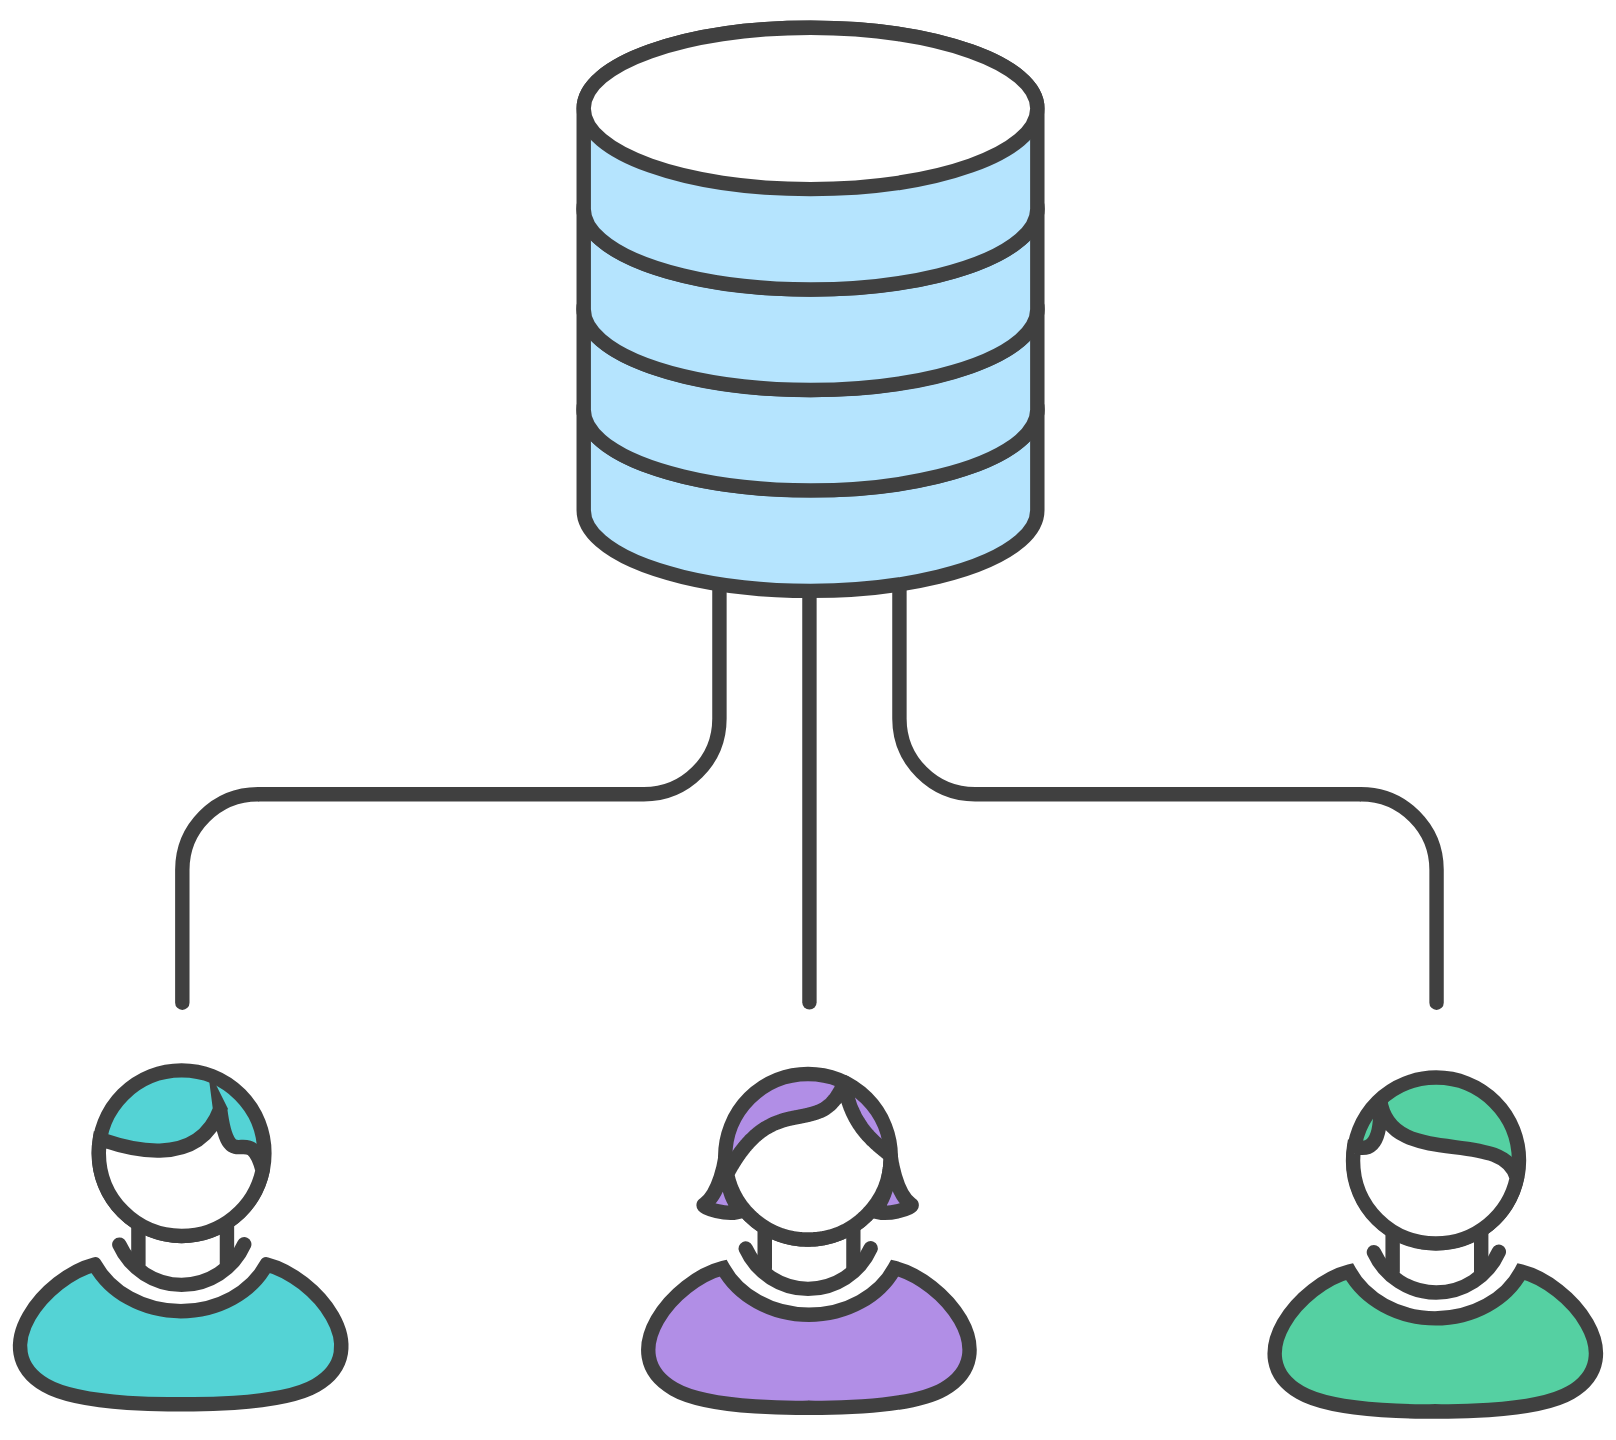
\includegraphics[scale=.15]{img/git-fluxo-centralizado.png}
\end{center}
}

\SliT{Fluxo de trabalho centralizado}{
\begin{itemize}

    \iOn{Não requer nenhuma outra ramificação além de \texttt{master}}

    \iOn{\textbf{O mais simples dos fluxos de trabalho}}

    \iOn{Como funciona:}

    \begin{itemize}
    
        \iTw{\texttt{clone} do repositório central}

        \iTw{Em cópias locais são feitas edições dos arquivos e confirmação das
            mudanças (\texttt{git add \& git commit})}

        \iTw{Fazer \texttt{push} da \textit{branch} \texttt{master} local para
            a cópia remota;}
    
    \end{itemize}

\end{itemize}
}

\begin{SliTC}{Fluxo de trabalho centralizado}
Exemplo:
\begin{CodeD}{bash}
$ git clone <algum repositorio>
# Edição de arquivos;
$ git add <arquivos modificados>
$ git commit -m "descrição rápida de modificações"
$ git push origin master
\end{CodeD}
\end{SliTC}


\SliT{Fluxo de trabalho centralizado}{
\begin{itemize}

    \iOn{Conflitos:}

\end{itemize}

\begin{center}
    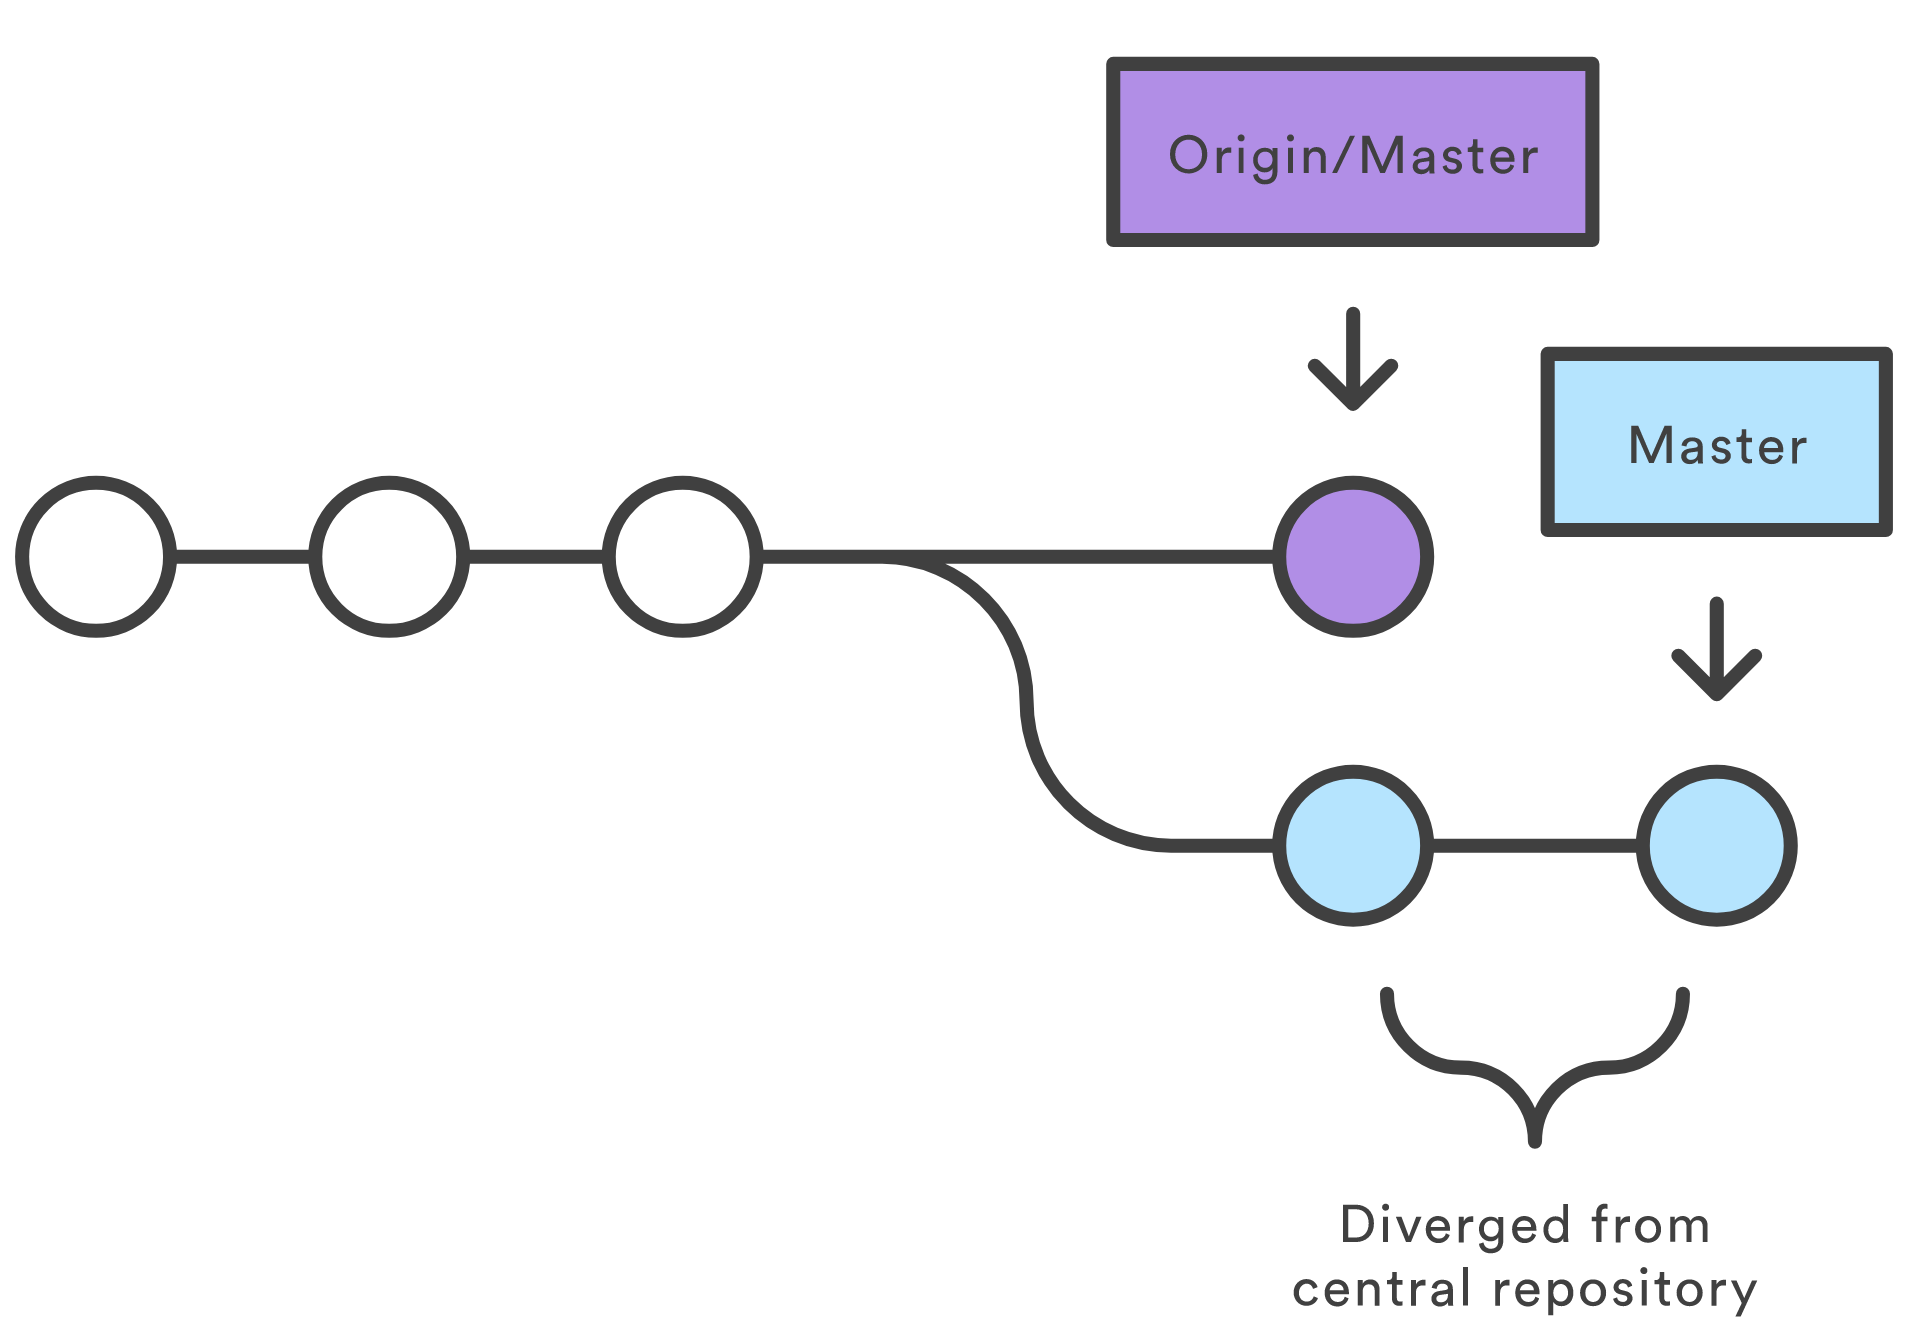
\includegraphics[scale=.2]{img/git-fluxo-centralizado-conflito1.png}
\end{center}
}


\SliT{Fluxo de trabalho centralizado}{
\begin{itemize}

    \iOn{Resolvendo conflitos (exemplo):}

    \begin{itemize}
    
        \iTw{John trabalha nas suas mudanças}
    
    \end{itemize}

\end{itemize}

\begin{center}
    
\includegraphics[scale=.2]{img/git-fluxo-centralizado-conflito2.png}
\end{center}

}


\SliT{Fluxo de trabalho centralizado}{
\begin{itemize}

    \iOn{Resolvendo conflitos (exemplo):}

    \begin{itemize}
    
        \iTw{Mary trabalha nas suas mudanças}
    
    \end{itemize}

\end{itemize}

\begin{center}
    
\includegraphics[scale=.2]{img/git-fluxo-centralizado-conflito3.png}
\end{center}

}


\begin{SliTC}{Fluxo de trabalho centralizado}
\begin{itemize}

    \iOn{Resolvendo conflitos (exemplo):}

    \begin{itemize}
    
        \iTw{John publica suas mudanças}
    
    \end{itemize}

\end{itemize}

\begin{center}
    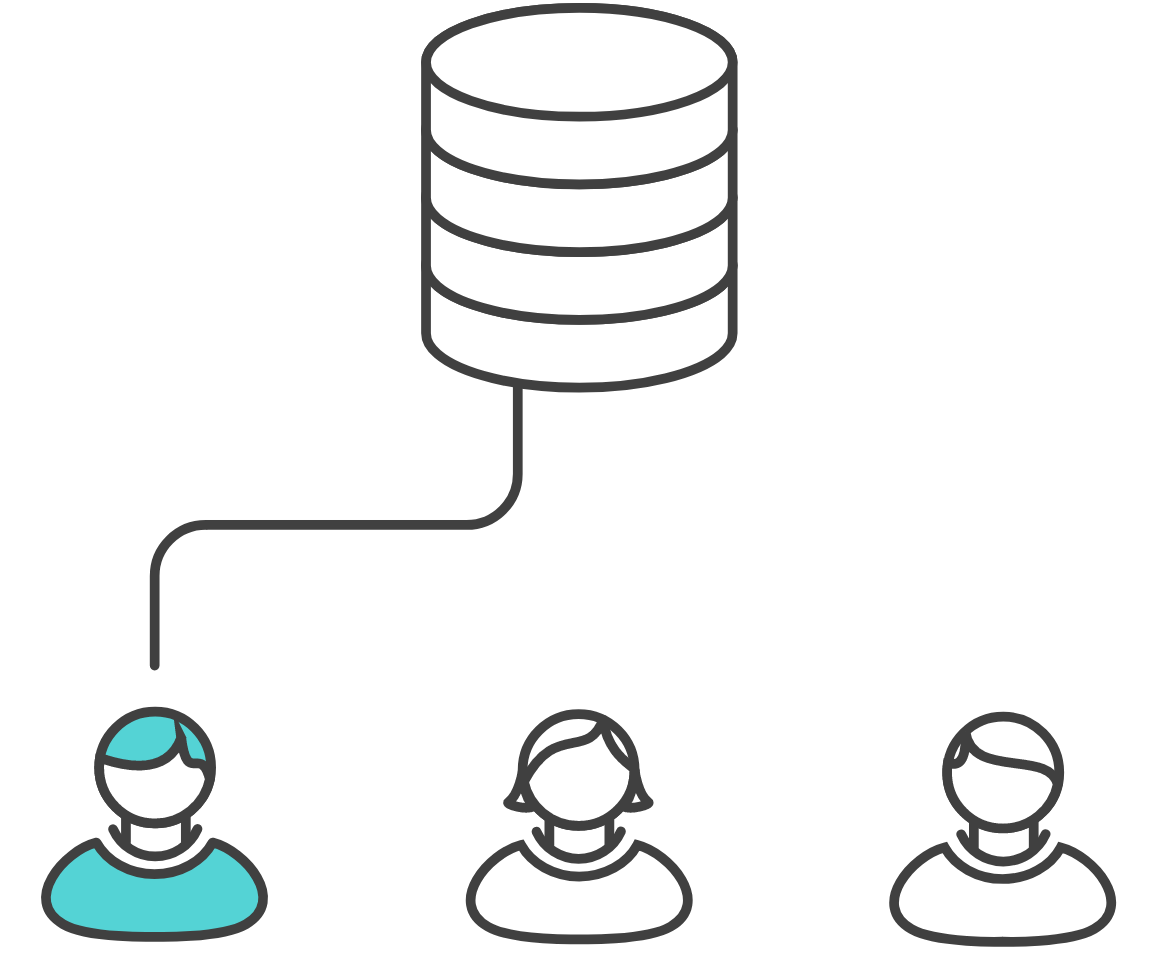
\includegraphics[scale=.2]{img/git-fluxo-centralizado-conflito4.png}
\end{center}

\begin{CodeD}{bash}
$ git push origin master
\end{CodeD}

\end{SliTC}


\begin{SliTC}{Fluxo de trabalho centralizado}
\begin{itemize}

    \iOn{Resolvendo conflitos (exemplo):}

    \begin{itemize}
    
        \iTw{Mary tenta publicar suas mudanças}
    
    \end{itemize}

\end{itemize}

\begin{center}
    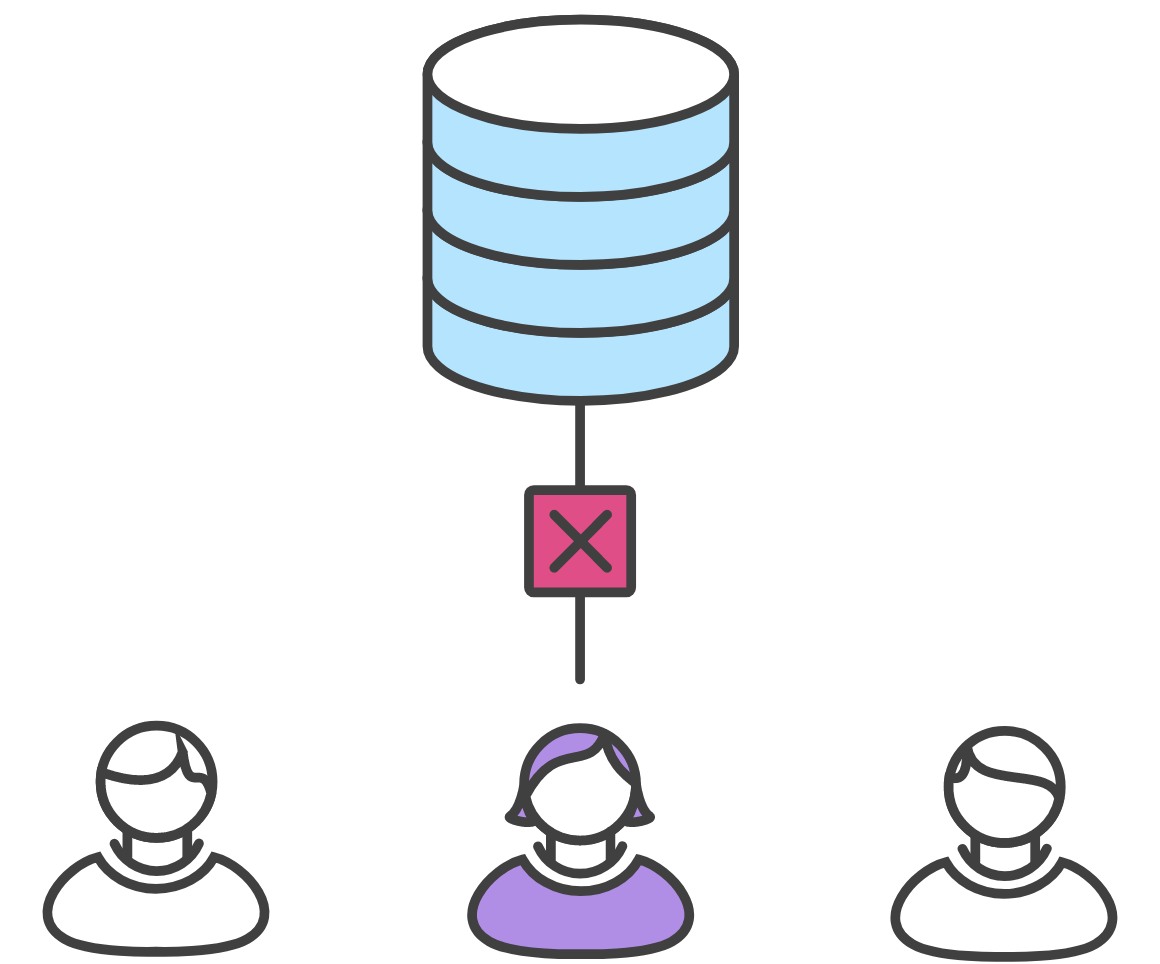
\includegraphics[scale=.2]{img/git-fluxo-centralizado-conflito5.png}
\end{center}

\begin{CodeD}{bash}
$ git push origin master
\end{CodeD}

\end{SliTC}


\begin{SliTC}{Fluxo de trabalho centralizado}
\begin{itemize}

    \iOn{Resolvendo conflitos (exemplo):}

    \begin{itemize}
    
        \iTw{Mary tenta publicar suas mudanças}
    
    \end{itemize}

\end{itemize}

\begin{CodeD}{bash}
 ! [rejected]        master -> master (fetch first)
error: failed to push some refs to '/Users/rocknroll/github/meu-repositorio'
hint: Updates were rejected because the remote contains work that you do
hint: not have locally. This is usually caused by another repository pushing
hint: to the same ref. You may want to first integrate the remote changes
hint: (e.g., 'git pull ...') before pushing again.
hint: See the 'Note about fast-forwards' in 'git push --help' for details.
\end{CodeD}

\end{SliTC}



\begin{SliTC}{Fluxo de trabalho centralizado}
\begin{itemize}

    \iOn{Resolvendo conflitos (exemplo):}

    \begin{itemize}
    
        \iTw{Mary faz o \texttt{rebase} de suas mudanças}
    
    \end{itemize}

\end{itemize}

\begin{center}
    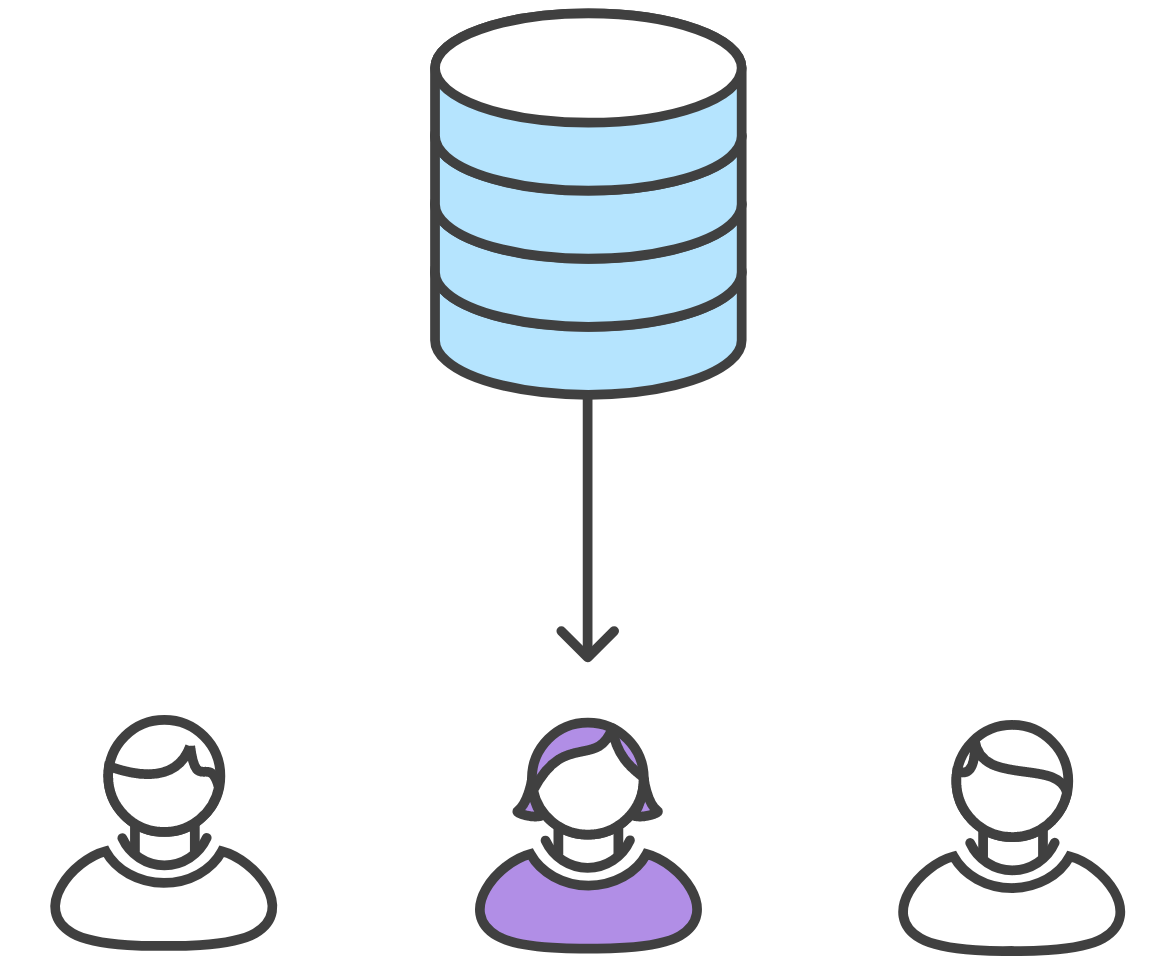
\includegraphics[scale=.2]{img/git-fluxo-centralizado-conflito6.png}
\end{center}

\begin{CodeD}{bash}
$ git pull --rebase origin master
\end{CodeD}

\end{SliTC}


\begin{SliTC}{Fluxo de trabalho centralizado}
\begin{itemize}

    \iOn{Resolvendo conflitos (exemplo):}

    \begin{itemize}
    
        \iTw{\texttt{--rebase} diz ao Git para mover todos os commits de Mary
            para a ponta da ramificação mestre}
    
    \end{itemize}

\end{itemize}

\begin{center}
    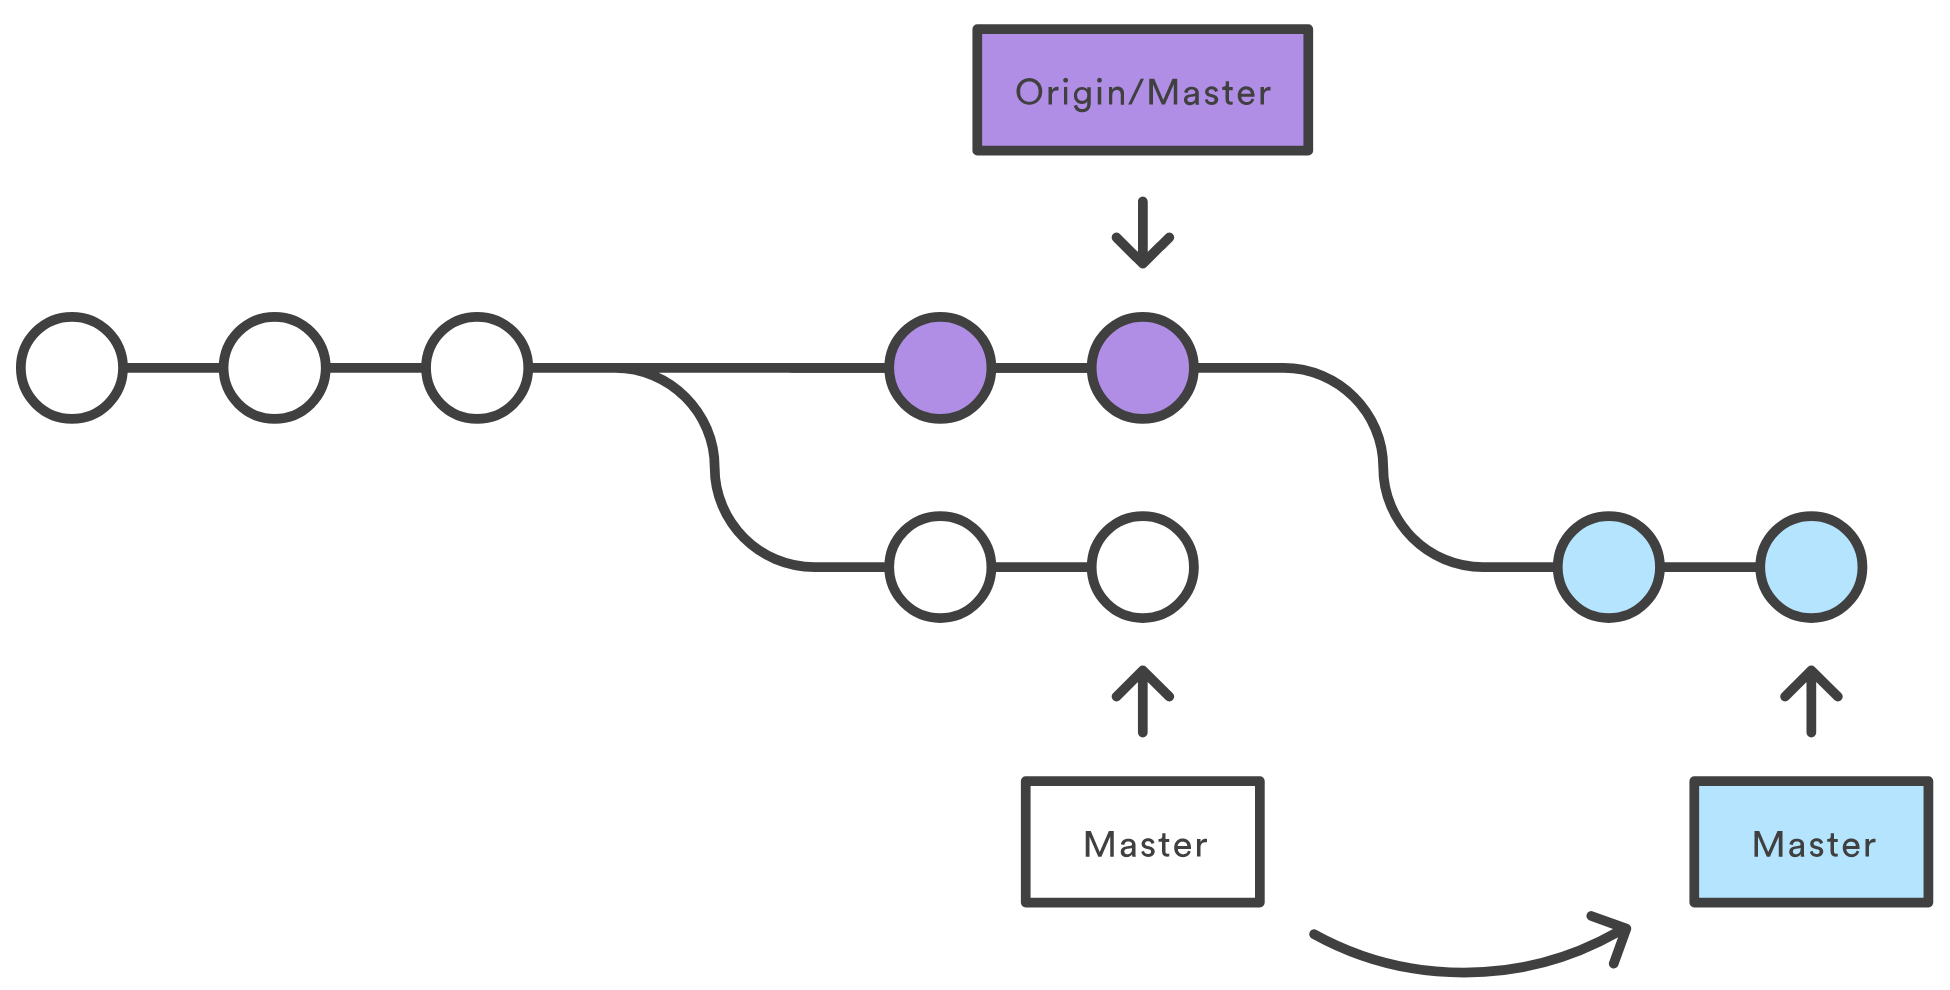
\includegraphics[scale=.25]{img/git-fluxo-centralizado-conflito7.png}
\end{center}

\end{SliTC}


\begin{SliTC}{Fluxo de trabalho centralizado}
\begin{itemize}

    \iOn{Resolvendo conflitos (exemplo):}

    \begin{itemize}
    
        \iTw{Se Mary e John estiverem trabalhando em recursos não relacionados,
            é improvável que o processo de rebase gere conflitos. }

        \iTw{se gerar, o Git vai pausar o rebase na confirmação atual e enviar
            a seguinte mensagem, juntamente com algumas instruções relevantes:}
    
    \end{itemize}

\end{itemize}

\begin{CodeD}{bash}
CONFLICT (content): Merge conflict in <file>
Resolve all conflicts manually, mark them as resolved with
"git add/rm <conflicted_files>", then run "git rebase --continue".
\end{CodeD}

\end{SliTC}


\begin{SliTC}{Fluxo de trabalho centralizado}
\begin{itemize}

    \iOn{Resolvendo conflitos (exemplo):}

    \begin{itemize}
    
        \iTw{Verificando o status no repositório de Mary}

    \end{itemize}

\end{itemize}

\begin{CodeD}{bash}
$ git status
Unmerged paths:
  (use "git restore --staged <file>..." to unstage)
  (use "git add <file>..." to mark resolution)
	both modified:   <file>
\end{CodeD}

\end{SliTC}


\begin{SliTC}{Fluxo de trabalho centralizado}
\begin{itemize}

    \iOn{Resolvendo conflitos (exemplo):}

    \begin{itemize}
    
        \iTw{Verificando o conflito no repositório de Mary}

    \end{itemize}

\end{itemize}

\begin{CodeD}{bash}
<<<<<<< HEAD
<Local File Content>
=======
<Remote File Content>
>>>>>>> Remote Repo Commit Message
<Common ContentL>
\end{CodeD}

\end{SliTC}




\begin{SliTC}{Ruby Code - Solarized Light Palette}
    \begin{CodeL}{ruby}
case node[:platform] # node info
when "debian", "ubuntu"
  package "git-core" # package is a resource
else 
  package "git"
end
    \end{CodeL}
    Texto
\end{SliTC}

\begin{SliTC}{Shell Code - Solarized Dark Palette}
    \begin{CodeD2}{bash}
#!/bin/bash
echo "Printing text with newline"
echo -n "Printing text without newline"
echo -e "\nRemoving \t backslash \t characters\n"
    \end{CodeD2}
\end{SliTC}


\begin{SliTC}{Python Code - Monokai Palette}
    \begin{CodeD}{python}
# Python Program to calculate the square root
# Note: change this value for a different result
num = 8 

# To take the input from the user
num = float(input('Enter a number: '))

num_sqrt = num ** 0.5
print('The square root of %0.3f is %0.3f'%(num ,num_sqrt))
    \end{CodeD}
\end{SliTC}


\SliT{Title}{
\secx{Section}

\secxx{Sub-Section}

% EXERCISE
\exe{4}{Exercise}
% SUGGESTED READING BOX			
\sug{References}
% CITATION						
\cittex{Citation}

}%%%%%%%%%%%%%%%%%%%%%%%%%%%%%%%%%%%%%%%%%%%%%%%%%%
% ###############################################################################
% SLIDE DOUBLE COLUMN WITH TITLE
\SliDT{Title}{First Column}{Second Column

}%%%%%%%%%%%%%%%%%%%%%%%%%%%%%%%%%%%%%%%%%%%%%%%%%%
% ###############################################################################
% SLIDE DOUBLE COLUMN NO TITLE
\SliD{
First Column}{
    { \begin{center}
    
\includegraphics[scale=0.35]{AI2Logo.png}     
    \end{center} }

}%%%%%%%%%%%%%%%%%%%%%%%%%%%%%%%%%%%%%%%%%%%%%%%%%%
% ###############################################################################
\end{document}
